\documentclass[MTech]{iitmdiss}
\usepackage{times}
\usepackage{epsf}
\usepackage{threeparttable}
\usepackage{setspace}
\usepackage{amsmath}
\usepackage{amsthm}
\usepackage{txfonts,pxfonts,amsfonts}
\usepackage{epsfig}	
\usepackage{caption}
\usepackage{subfig}
\usepackage{listings}
\usepackage{epstopdf}
%\usepackage[dvips]{graphicx}
\usepackage{graphicx}
%\usepackage{pstricks,pst-node,pst-tree,pstricks-add}
% \usepackage[square,numbers,sort]{natbib}
\usepackage[square]{natbib}
\usepackage{hyperref}
%\usepackage[hypertex]{hyperref} % hyperlinks for references.
%\usepackage{algorithmic}
%\usepackage{algorithm}


%\include{commands}

% Strut macros for skipping spaces above and below text in tables. 
\def\abovestrut#1{\rule[0in]{0in}{#1}\ignorespaces}
\def\belowstrut#1{\rule[-#1]{0in}{#1}\ignorespaces}

\def\abovespace{\abovestrut{0.20in }}
\def\aroundspace{\abovestrut{0.20in}\belowstrut{0.10in}}
\def\belowspace{\belowstrut{0.10in}}
%%%%%%%%%%%%%%%%%%%%%%%%%
\def\thesistitle{Video Event Localization and Identification}
\def\thesisauthor{G K Sudharshan}

\begin{document}
\bibliographystyle{iitm}
%%%%%%%%%%%%%%%%%%%%%%%%%%%%%%%%%%%%%%%%%%%%%%%%%%%%%%%%%%%%%%%%%%%%%% 
% Title page

\title{\thesistitle}
\author{\thesisauthor}

\date{May 2015}
\department{Computer Science and Engineering}

%\nocite{*}
\begin{singlespace}
\maketitle 
\end{singlespace} 



%%%%%%%%%%%%%%%%%%%%%%%%%%%%%%%%%%%%%%%%%%%%%%%%%%%%%%%%%%%%%%%%%%%%%%
% Certificate
\certificate
\vspace*{0.5in}
\noindent This is to certify that the thesis entitled {\bf {\thesistitle}}, 
submitted by {\bf {\thesisauthor}}, to the Indian Institute of Technology, 
Madras, for the award of the degree of {\bf Master of Technology}, 
is a bonafide record of the research work carried out by him under my
supervision. The contents of this thesis, in full or in parts, have not been
submitted to any other Institute or University for the award of any degree or diploma.
\vspace*{1.4in}
\hspace*{-0.25in}
\begin{singlespace}
\noindent {\bf Prof.~Hema~A~Murthy} \\
\noindent Research Guide \\ 
\noindent Professor \\
\noindent Dept. of Computer Science and Engineering\\
\noindent IIT-Madras, 600 036 \\
\end{singlespace}
\vspace*{0.20in}
\noindent Place: Chennai\\ 
Date:


%%%%%%%%%%%%%%%%%%%%%%%%%%%%%%%%%%%%%%%%%%%%%%%%%%%%%%%%%%%%%%%%%%%%%%
% Acknowledgements
\acknowledgements
I would like to to express my sincere thanks and deep sense of indebtedness to my guide Prof. Hema A.  Murthy for her guidance and motivation throughout my work.  Her inspiring suggestions motivated me to solve problems efficiently.  I am also grateful to my guide also for providing access to the DONLAB servers: Dell-d1 and Dell-d2 without which none of my experiments could have been performed.

\par I would like to thank my partner Abil N George for his support and contribution in the toolkit development.  Also my deepest gratitudes to Prof. C. Chandra Sekhar and Anil Kumar Chilli for allowing us to use systems with GPU in the Speech and Vision Laboratory during the development of the toolkit. 

\par Also I would like to acknowledge all my colleagues at DONLAB (IIT Madras) who have helped me throughout my research. 
 
\par Lastly, I am thankful to my parents for all the moral support and the amazing oppurtunities they have given me over the years.

%%%%%%%%%%%%%%%%%%%%%%%%%%%%%%%%%%%%%%%%%%%%%%%%%%%%%%%%%%%%%%%%%%%%%%

%%%%%%%%%%%%%%%%%%%%%%%%%%%%%%%%%%%%%%%%%%%%%%%%%%%%%%%%%%%%%%%%%%%%%%
% Abstract
\abstract

\noindent KEYWORDS: \hspace*{0.5em} \parbox[t]{4.4in}{Convolutional Neural Network; Spatio Temporal Volume; Background Subtraction; Saliency Estimation; Temporal Smoothening}

\vspace*{24pt}
In last few years because of the digitization there have been breakthrough on volume of videos accessible, but all become worthless if they are not refined into some application. One such application is a real time event recognition which has been a fundamental research arena in the vision domain. It aims to recognize the actions and goals of multiple subjects from a given sequence of frames. The major challenges with real time event recognition are geometric and photometric variances, clutter background and complex camera motion. Most of the current solutions are based on extracting complex hand-crafted features, but these features does not work in all scenarios and is a tedious process. 

\par Hence a problem has been set by dimidiating it into event localization and event recognition task by isolation of all possible event regions in given train of frames and then predicting. 

\par Just like social localization where social network users are connected based on interest and hobbies of a individual, video event localization intends to connect pixels or regions showing similar color, texture and motion characteristics.  This was accomplished by an endemic approach to obtain visual attention score (VAS) by fusing background subtraction (procure pixels that alter in subsequent frames) and saliency estimation (derive objects in frame) . The background subtraction extract pixels that are inmotion while saliency  derive important regions based on color and texture attributes. Also a  novel method was proposed for temporal smoothening of the visual attention score  with the motivation to obtain a similar region in subsequent frames. This is important because VAS may be vulnerable to sudden camera motion and illumination variances.  Window tracking is supplemented over the temporal smoothening to obtain a bounding box that correspond to an event. These bounding boxes are termed as spatio temporal volume (STV). The STV extracted from video segments are supplied to a CNN to identify the corresponding event label.

\par As part of event recognition an indigenous deep neural network toolkit was built using external libraries. Though the toolkit encompass of different techniques, only convolutional neural network (CNN) was exploited as it is acclaimed for image classification. 
%Also investigation were done on providing  processed features as input along with the raw images to CNN.

\par Highlights of this approach include state of the art results for standard UCF-50 video dataset and an indigenous and innovative method for solving various problems like surveillance, video summarization and more.  
\pagebreak
%%%%%%%%%%%%%%%%%%%%%%%%%%%%%%%%%%%%%%%%%%%%%%%%%%%%%%%%%%%%%%%%%
% Table of contents etc.
\begin{singlespace}
\tableofcontents
\thispagestyle{empty}
\listoftables
\addcontentsline{toc}{chapter}{LIST OF TABLES}
\listoffigures
\addcontentsline{toc}{chapter}{LIST OF FIGURES}
\end{singlespace}
%%%%%%%%%%%%%%%%%%%%%%%%%%%%%%%%%%%%%%%%%%%%%%%%%%%%%%%%%%%%%%%%%%%%%%
% Abbreviations
\abbreviations
\noindent 
\begin{tabbing}
xxxxxxxxxxx \= xxxxxxxxxxxxxxxxxxxxxxxxxxxxxxxxxxxxxxxxxxxxxxxx \kill
\textbf{CAB} \> Context Aware Based \\
\textbf{CNN}   \> Convolutional Neural Network \\
\textbf{ES} \> Eigen Subtraction \\
\textbf{FD} \> Frame Differencing \\
\textbf{HCB} \> Hierarchical Color Based \\
\textbf{MLP}   \> Multilayered Perceptron \\
\textbf{MOG} \> Mixture of Gaussian \\
\textbf{RC} \> Region Contrast \\
\textbf{SDB} \> Spectral Distribution Based \\
\textbf{STV} \> Spatio Temporal Volume \\
\textbf{VAS}   \> Visual Attention Score \\
\end{tabbing}



%%%%%%%%%%%%%%%%%%%%%%%%%%%%%%%%%%%%%%%%%%%%%%%%%%%%%%%%%%%%%%%%%%%%%%
%Notation

% \chapter*{\centerline{NOTATION}}
% \addcontentsline{toc}{chapter}{NOTATION}
 
% \begin{singlespace}
% \begin{tabbing}
% xxxxxxxxxxx \= xxxxxxxxxxxxxxxxxxxxxxxxxxxxxxxxxxxxxxxxxxxxxxxx \kill
% \textbf{$r$}  \> Radius, $m$ \\
% \textbf{$\alpha$}  \> Angle of thesis in degrees \\
% \textbf{$\beta$}   \> Flight path in degrees \\
% \end{tabbing}
% \end{singlespace}
 
% \pagebreak
% \clearpage

%The main text will follow from this point so set the page numbering
%to arabic from here on.
\pagenumbering{arabic}

 
%%%%%%%%%%%%%%%%%%%%%%%%%%%%%%%%%%%%%%%%%%%%%%%%%%
 % Chapters.
 \chapter{INTRODUCTION}
\label{chap:intro}
In the era of Google glass \citep{googleGlass}, %people wants everything in front of them to be explicable.
everybody wants everything, including video to be explained.  Just like in football, one would like to obtain the highlights of a match in terms of statistics, such as duration of ball control by respective team and more.  While in the sphere of surveillance, detecting multiple simultaneous events is very crucial.  All these tasks are broadly categorized as an application of video event recognition. 

\par A video event is defined as \textit{a fact or process of doing things to attain a goal}.  The video events may be short like a player kicking the ball or long as player scoring a goal.  It is noticed that most of the annotated events available are short events, also long events can be modelled as sequence of short events.  Only short events are considered in this work.  While the subject of event can be any physical objects like human, ball etc.
\par The problem of video event recognition is generally framed as prediction of video event from given set of labelled internet videos, where the label specifies the events that occurs within video.  But most of the datasets available are in weakly labelled settings, i.e they do not have spatio-temporal segmentation indicating coordinates and time points where and which event occurs.  Therefore the particular problem can bifurcated as localization and prediction problem.  The localization aspect of the problem is the task of locating the event within the video %and further build train of frame corresponding to the event
and then building a sequence of frames.  The train of frames correspond to the spatio temporal volume (STV) and are used by models for the prediction.
\par Even though the recognition appears to be simple there are quite a lot of challenges.  Most of the challenges observed are centred around the source of the video like dynamic background, moving camera, low lighting and more.  Another challenging aspect of this problem is to deal with large intra-category variations for achieving satisfactory classification on wide scale of videos.
\par Generally, such problems are tackled in the following manner : local feature extraction, feature aggregation, finally a classifier (such as SVM) to distinguish among the visual classes of interest.  But these approaches suffer from one major challenge, namely, the choice of feature that best represents video.  In last few years, deep neural network has revolutionized the machine learning field and has edified a new approach for training.  In the case of deep neural network, it accepts raw input rather than the processed features and generates (bottleneck) features in process of prediction. 
\par Convolutional neural network (CNN), a deep learning method has shown remarkable success for the visual recognition task as it takes advantages of the spatial structure of images/videos.  It was also observed resistant to translational variances and also supported several regularization tricks for address the large intra-category variances.  Therefore the CNN's are considered for  the event recognition problem.

\clearpage
\section{Outline of the Work}
A novel solution to the problem of video localization and recognition has been proposed. In the approach the input video is given to background subtraction to measure variation in pixel intensity in continuous frames.  Also the saliency measure is obtained for train of frames that capture the regions in the frame that are quite distinct in the frame.  Both the measure are fused to obtain a new score termed visual attention score (VAS) that can capture the motion as well as the contrast in given frame. 
\par CNN is being considered for event recognition which expects fixed size raw image/video as input. Therefore a spatio temporal volume (STV) corresponding to video event are extracted by smoothening the VAS to obtain bounding box that is being tracked along the sequence of frames.  Figure \ref{fig:outline} depicts the outline of the proposed solution to the event recognition problem.
\begin{figure}[htpb]
   \begin{center}
	    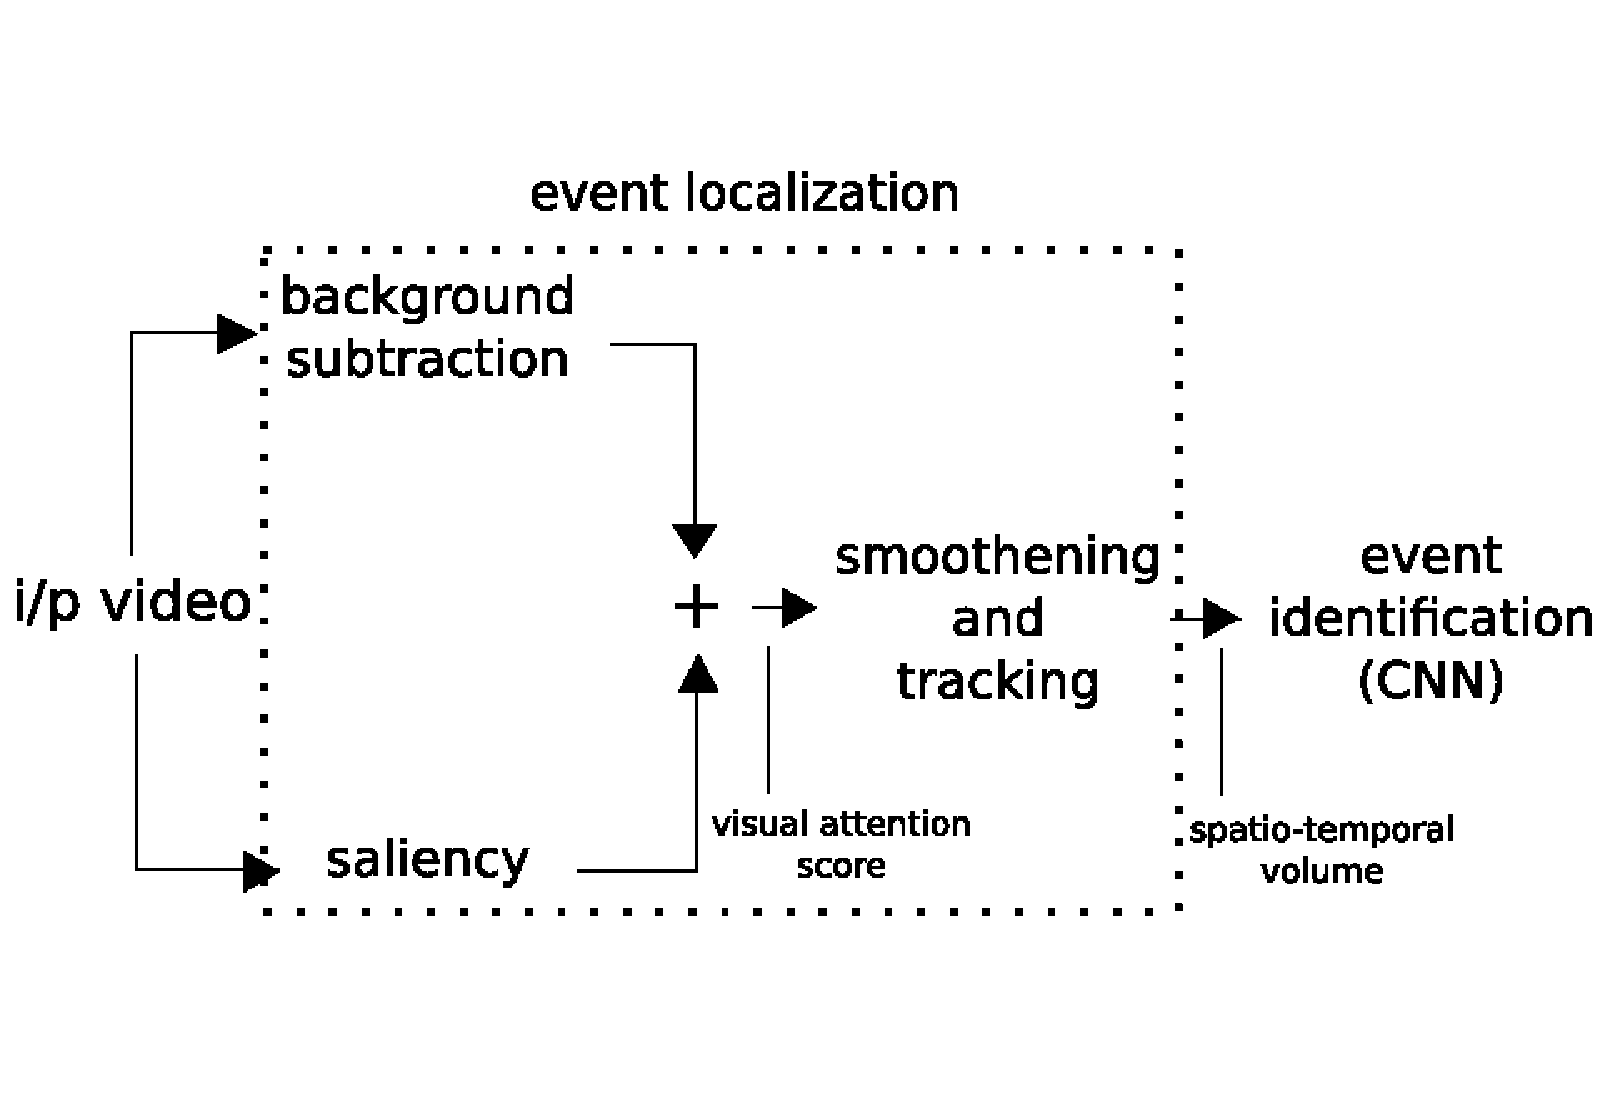
\includegraphics[width=0.95\textwidth]{snaps/outline.eps}     
     \caption {Proposed solution for video event recognition}
   \label{fig:outline}
   \end{center}
 \end{figure}
 
\section{Major Contribution}
\begin{itemize}
	\item{Built a indigenous deep neural network toolkit providing an ease to configure for different neural network models.}
	\item{Proposed a novel approach to obtain visual attention score by fusing the background subtraction and saliency measure.}
	\item{Suggested different ways for performing temporal smoothening over the visual attention score by considering a temporal context.}
	\item{Devised algorithm for extracting spatio temporal volume from the smoothed scores.}
\end{itemize}

\section{Organization of thesis}
\par Chapter \ref{chap:eventrec} includes discussion about the existing techniques used for event recognition and the home-grown implementation of neural network.  While in chapter \ref{chap:eventLo} steps for extracting spatio-temporal volume by fusing background subtraction and saliency measure is being elaborated.  The experiments for the event recognition and the justification for choosing the appropriate techniques for the ultimate model are chalked in chapter \ref{chap:exp}.  The future scope and the summary of the entire work can be seen in chapter \ref{chap:concl}.
\chapter{EVENT LOCALIZATION}
This section of thesis considers the problem of localization: the objective is to detect where an action of interest occurs. The expected output of such a system is typically a subvolume encompassing the action of interest. Since a localized action only covers a fraction of the spatio-temporal volume in a video, the task is considerably more challenging than event classification. Some of the common startergies that are tried on this kind of problems are efficient sub-window search ~\citep{subwindowsearch},"selective search" stratergy ~\citep{selectivesearch}  and a recent by ~\cite{tubelet}, but these either does a exhaustive search or does a iterative merging of the supervoxels. 

\section{Background Subtraction Techniques} 
\par Event localization can be performed by determining the position with pixel changes and understanding the motion relativity ~\citep{Basharat08}, where all components corresponding to an event show a similar flow of pixels. Following approach works significantly well in surveillance data but fails terribly in case human event detection. Later realized that, by eliminating the background(static parts) of the visual frame,  possible event locations can be retained.  Several background subtraction technique are eminent in the \cite{Piccardi04}, among these some apply on static image while others on dynamic video. In case of our application we can blend both these approaches to generate more reliable event detectors.

\subsection{Frame Differencing (FD)}
A very common approach for performing the moving object segmentation is using frame differencing but these approach is very sensitive to small changes and yields lots of noise when a camera is in motion. A simplest way to implement this technique is by computing the absolute difference of gray scale/intesity values two consecutive frames. Consider $P(p_x,p_y,t)$, intesity of pixel $(p_x,p_y)$ at frame t, then pixel $(p_x,p_y)$ that is considered foreground when absolute difference is above a threshold,$$\vert P(p_x,p_y,t+1) - P(p_x,p_y,t)t\vert > T$$.
\par The robustness of this method depends on speed of forground elements. Faster movements may require higher thresholds to reduce the noise.  An alternate approach is to replace difference of a single previous frame  by an average of multiple previous frames, still results are noisy and not reliable.

\subsection{Eigen subtraction (ES)}
An alternate approach named eigen background subtraction was seen to be more elegant. A sample of N images of the videos are obtained, mean background image $\nu_b$ is computed and all images are mean normalized  $X$. Principal component analysis on the mean normalized images is performed , idea is, that a high-dimensional images are often described by correlated variables and only a few meaningful dimensions account for most of the information. But performing PCA is not straightforward, consider 100 images of dimension 100x100 pixels, then the dimension of generated covariance matrix would be 10000x10000, i.e roughly 0.8 GB (considering 64 bit float values). Solving this is not feasible, hence a trick from linear algebra that for a MXN matrix with $M>N$, can at most have N-1 non-zero eigen values ~\cite{Duda01} can be used. Eigen decomposition of $X^TX$ is carried out:
$$X^TX\nu_i=\lambda_i\nu_i$$
$$XX^T(X\nu_i)=\lambda_i(X\nu_i)$$
The orthonormal eigen vector of $XX^T$ is found out by normalizing $X\nu_i$ to unit length. Once eigen vectors of $XX^T$  are computed, projection of the current frame $F$ on the eigen vector with top eigen values are determined, and the reconstructed frame $F'$ is obtained by using the projection coefficients and the eigen vectors. The difference $F-F'$ would correspond to the mask on the moving object. 

\subsection{Mixture of Gaussian (MOG)}
This is one of the well known method of extracting foreground information. \cite{kaew} model each background pixel by a mixture of N Gaussian distributions. The weights of the mixture represent the time proportions that those colors stay in the scene. The probable background colors are the ones which stay longer and more static. At any instance $i$ a particular pixel $(p_x,p_y)$ has color space represented as $V(p_{x},p_{y},i)$, history of the pixels are given by 
$$X_{1},..,X_{t} = {V(p_{x},p_{y},i)~:~1\le i \le t }$$
The history is modeled by mixture of N gaussian mixtures,
$$P(X_{t})=\Sigma_{i}^{N}w_{(i,t)}\eta(X_{t},\mu_{(i,t)},\Sigma_{(i,t)})$$
\par $w_{(i,t)}$,$\mu_{(i,t)}$,$\Sigma_{(i,t)}$ are weight,mean and covariance of the $i^{th}$ Gaussian in the mixture at time $t$ respectively and where $\eta$ is gaussian density function. General principle behind this approach is that when a new object occludes the background object, it will not match one of the existing distributions. Instead will result in either the creation of a new distribution or the increase in the variance of an existing distribution. The variance of the moving object is expected to remain larger than a background pixel until the moving object stops.
\begin{figure}[htpb]
   \begin{center}
	    \includegraphics[width=0.75\textwidth]{snaps/bgsub/results.eps}     
     \caption {Background subtraction techniques on multiple video classes}
   \label{fig:bgsub}
   \end{center}
 \end{figure}
\par Results of foreground mask obtained using moving average, eigen subtraction methods and mixture of gaussian are shown in Figure \ref{fig:bgsub}. 



\section{Saliecny Detection}
Visual saliency is the distinct subjective perceptual quality which makes some items in the world stand out from their neighbors and immediately grab our attention.
As we had discussed earlier about the different techniques to extract the eminent pixels which are in motion, sometimes pixels which are stationary and quite distinct might also play a important role in the the activity recognition. These approaches are considered during the process attention modelling. Most of saliency estimations techniques in literature have got a common process,
\begin{enumerate}
	\item{\textbf{Color equalization:} It is done by removing the tail in the color histogram. This helps to improve the contrast in an image. In our implmentation color equalization is done on each channel separetely so that all channels can be provided to the clustering algorithm.}
	\item{\textbf{SLIC-based segmentation:}  It is a simple linear iterative clustering that clusters pixels in the combined five-dimensional color and image plane space to efficiently generate compact, nearly uniform superpixels. Any slic based clustering algorithm takes two parameters number of super-pixels and compactness of each superpixel. According to \cite{slic}, slic is fastest and most memory efficient compared to  other segmentation technique like graph-cut, quick shift segmentation technques. Segmentation reduces the number of computation in the subsequent stages}
	\item{\textbf{Extract segment properties:} Extracting features of the region that are used in computing the saliecny of each regions. Some features that are considered in our implementation are color based features (LAB,RGB) and texture based features (GLCM,Texture Flow).}
	\item{\textbf{Compute~saliency:} Saliecny estimation techniques can be broadly categprozed into bottom-up, top-down and information maximization based on algorithmic computation. Earliest saliency based attention modelling was proposed by \cite{itti}. It was inspired by the behavior and the neuronal architecture of the early primate visual system.}
	\item{\textbf{Saliency cut:} Saliency maps are generally thresholded to obtain the salient mask. In the implementation, grab-cut\citep{grabcut} performs segmentation by modeling foreground and background based on saliency estimation to obtain the mask. We considered higher saliency  correspond to foreground while lower saliency correspond to background. After getting the saliency mask we apply few morphological operation to remove the salt and pepper noise}
\end{enumerate} 
\par Some of the distiguished saliency estimation techniques are discussed below. 
\subsection{Hierarchical Color Based}
It is a top-down approach for computing saliency. In this approach we hierarchically set saliency map of improbable salient pixels to zero. The hierarchy is based on the neighborhood window size. 

\subsection{Contxt Aware Based}
\subsection{Spectral Distribution Based}
\subsection{Regional Contrast}




\chapter{EVENT IDENTIFICATION}
 \label{chap:eventrec}
 \section{Introduction}
Visual event identification has been observed as a potential area of research in several applications like  content-based video retrieval, human computer interaction, etc..  In general, the visual event identification is always modelled as a stochastic temporal processes in the semantic space.  The motivation behind this is to capture the dynamic patterns of event through collective evolution of the semantic concept.  One of the most familiar methods that use this approach is that of Hidden Markov Model (HMM), which has been a favourite for sequential pattern recognition.  However, the HMMs have struggled to incorporate both the spatial and temporal context present in the event.  
\par In another approach by ~\cite{YanKe05}, the event is treated as a space-time volume in the video sequence.  Volumetric features based on optical flow are extracted for event detection.  These are generally used for videos having only single moving object (human) and action.  For complex activity recognition \citep{YanKe07}, the internet videos are already temporarily localized and they focus on identifying the primitive event.
\par A common approach for video classification ~\citep{Liu09}~\citep{Niebles10} involves : extracting local region level features, combining features to fixed size video level description and training a classifier on the features to predict the class labels.  But in these approaches, feature extraction plays a crucial role, and features must be recomputed again for different videos.  Convolutional Neural Network (CNN) replace all three stages with a single neural network ~\cite{Ji13},  and is trained end-to-end from the raw pixel values to classifier outputs. However, CNNs were observed to be computationally expenisve and took longer training periods to effectively optimize the solution.  With the improvements on GPU hardware, CNNs could be scaled to train networks of millions of parameters.

\par Section \ref{sec:cnn} outlines the overall framework of CNNs and discusses the reasons for choosing it for the event identification task over the existing techniques.  Then, we will elaborate the architecture and features supported by the indigenous deep neural network tool kit designed in python in Section \ref{sec:pyDNN}. 

\section{Convolutional Neural Network (CNN)}
 \label{sec:cnn}
 \par Convolutional neural networks (CNN) are a variant of multi-layer perceptron (MLP) that are designed by studying the complex arrangement of cells in the cat's visual cortex.  It comprises of one or more convolutional layers (often with a sub-sampling step), followed by one or more standard MLPs.  There are different varieties of CNN based on the dimensionality of input and convolution operator like CNN-2D, CNN-3D etc.  Figure \ref{fig:cnnarchitecture} depicts a sample CNN architecture with two convolution and subsampling layers followed by a single MLP layer.
 
\begin{figure}[htpb]
   \begin{center}
   		{%
			\setlength{\fboxsep}{5pt}%
			%\setlength{\fboxrule}{1pt}%
	    		\fbox{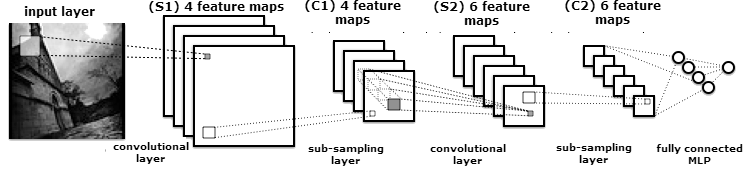
\includegraphics[width=0.98\textwidth]{snaps/cnn.png}}  
	    }%
     \caption[] {A sample CNN architecture \footnotemark}
	\label{fig:cnnarchitecture}  
   \end{center}
 \end{figure} 
\par A major advantage of having CNN is that it learns faster (fewer parameters) compared to MLP with the same number of hidden units.  CNN  also uses gradient based optimization to compute the parameters of the model.  It has been shown that CNNs fits very well onto the visual recognition domain, as it handles very high dimensional data, exploits the topology of image or video, and is invariant to small translation and illumination changes.  CNN leverages the following concepts to tackle the above mentioned challenges:
\footnotetext{\url{http://deeplearning.net/tutorial/lenet.html}}
\subsection{Local Connectivity}
It exploits the spatially local correlation, allowing only local connectivity between neurons of adjacent layers.  Hence, every hidden unit is only sensitive to a small block in the visual field called the receptive field. This drastically reduces the number of connections between the input and the hidden layer which therefore diminishes the number of parameters needed to train the model.
\subsection{Shared Filters}
The hidden units are associated to the receptive field by filters which are shared within a feature map. These filters capture edge like patterns within the receptive field.  Additionally, sharing filters increases the learning efficiency by greatly reducing the number of free parameters to be learned.  Apart from reducing parameters, they extract the same feature at every position, which makes every feature map to be equi-variant to any changes in the input.  The shared filters are associated to the receptive field by a dot product operation which can be expressed as a discrete convolution operation.
\subsection{Pooling/Sub-sampling Hidden Units}
The sub-sampling layer pools the hidden unit output in the non-overlapping neighbourhood.  Pooling can be either average or maximum.  The max-pooling provides local translation invariance and is commonly used.  Pooling also reduces the inputs to the next layer of feature extraction.  With pooling, the feature maps in the latter layer extract coarser features.

\par All these concepts empower CNNs to achieve better generalization in vision problems.  Stacking multiple such layers is a very common approach to attain better responsiveness over a larger visual field.  Some architectural tricks such as rectification and contrast normalization are tried for improving result on large dataset.  The unsupervised pre-training of each filter weight has helped enhance the robustness of the models built.

\section{Python-DNN Toolkit}
\label{sec:pyDNN}
Neural networks can be best implemented using a modular, object-oriented approach,  Where each of the models (DNN, SdA, CNN) are implemented as different classes with member functions performing pre-training (an unsupervised learning), fine-tuning (supervised learning), testing , loading and saving the model.  This approach enables reuse of the code for most of the network models.  Even though the most of the existing toolkits are quite sophisticated, these toolkits are reasonably hard to configure. They needed to be configured either through the command line or by providing the necessary arguments to a function.  Since neural networks take too many parameters, it gets difficult to understand the purpose of any given parameter.  Hence, the \textit{Python-DNN} toolkit was developed.  
\subsection{Architecture}
The toolkit was implemented in python using the numerical computation library named \textit{Theano} \citep{theano}.  It provides a platform to run our toolkit efficiently in both CPU and GPU architecture.  Architecture of the indigenous DNN toolkit is shown on \ref{fig:architecture}.
\begin{figure}[htpb]
   \begin{center}
   		{%
			\setlength{\fboxsep}{5pt}%
			%\setlength{\fboxrule}{1pt}%
	    		\fbox{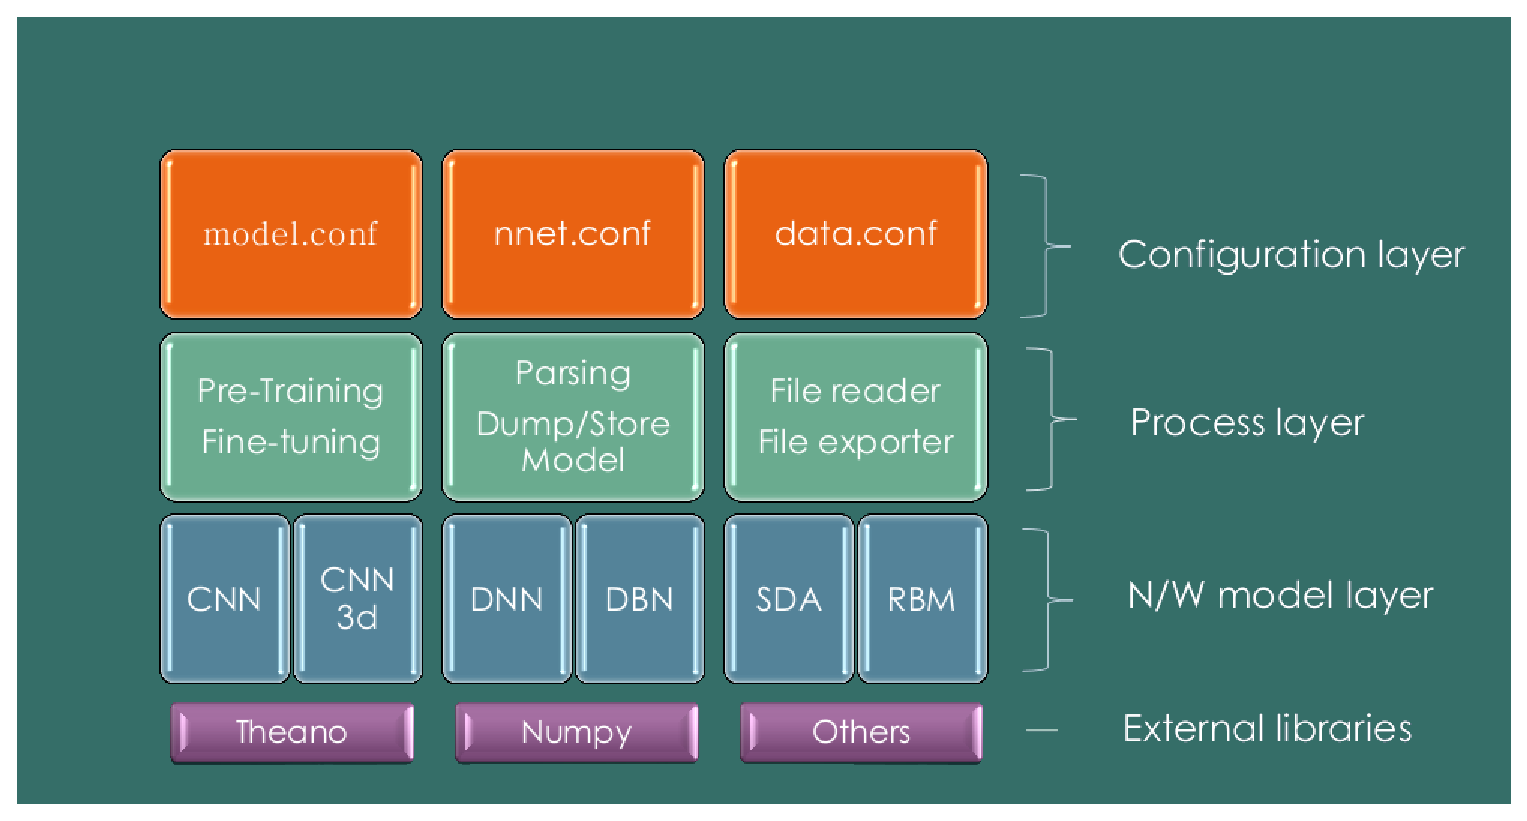
\includegraphics[width=0.90\textwidth]{snaps/colorarchitecture.eps}}  
	    }%
     \caption {Python-DNN architecture}
	 \label{fig:architecture}
   \end{center}
 \end{figure}
Toolkit has been split into four layers : external libraries that include all the dependent libraries, a network model layer that encompass different supervised and unsupervised models supported, a processing layer which focusses on the different operations supported by the different models and the topmost layer configuration layer is the input to the model.  The configuration layer contains three main configurations : 
 \begin{itemize}
	\item {\textbf{model.conf :} it constitute type of model, input model, output model, batch-size, number of outputs(classes), learning rate, momentum and more}
	\item {\textbf{nnet.conf :} it defines a neural network model like number of layers, number of nodes per layer, activation function}
	\item {\textbf{model.conf :} it constitutes a type of model, input model, output model, batch-size, number of outputs(classes), learning rate, momentum and more}
 \end{itemize}
The fine-tuning operation corresponds to the normal back propagation algorithm while the pre-training corresponds to greedy layer-wise learning.  This unsupervised learning at each layer in a way preserves information from the input and disentangles factors of variation.  Sample configurations for some well known datasets like MNIST and CIFAR are also made available with it.
\subsection{Salient Features}
\begin{itemize}
	\item Allows easy configuration of the model, configurations are organized in JSON format thus making the configuration legible to humans.
	\item Supports several types of data readers/writers. 
	\item Enables us to dump bottleneck features for their use in other applications.
	\item Incorporates activation functions : tanh, sigmoid, relu, cappedrelu
	\item Includes drop-out and regularization to tackle over fitting.
	\item Facilitates in loading pre-trained model and dumping the trained model.
	\item Encompass two and three dimensional convolutional models.
	\item Supports pre-training through stacked denoising autoencoders (SdA) and restricted boltzman machine (RBM).
	\item Runs efficiently in CPU and GPU architectures.	
\end{itemize}
Our implementation is publicly made available in github\footnote{\url{https://github.com/IITM-DONLAB/python-dnn}}.  Further details about the the toolkit like installation, configuration and its usage is explained in Appendix \ref{app:pydnn}. This toolkit was built together with Abil N George.
\clearpage

\section{Summary}
The CNN is versatile and yet conceptually simple, and has been adapted for a wide spectrum of cognitive tasks.  It takes advantage of the 2D/3D structure of an input image (or spectrogram in the case of speech signal) by using local connections and shared weights and provides for translational invariance by sub-sampling the layer outputs.  The ready-to-use indigenous toolkit supporting CNN helps in performing the experiments for event identification with ease.  In the next chapter, the experiments on different techniques for the event recognition will be elaborated.
\chapter{EXPERIMENTAL RESULTS}
\label{chap:exp}
This chapter justifies the reason for choosing appropriate set of techniques for event recognition based on  experiments conducted. The first stage of the task involve localization, which incorporate background subtraction, saliency estimation and temporal smoothening as discussed in Chapter \ref{chap:eventLo}. Evaluation of background subtraction was done intuitively, among the techniques frame-differencing was chosen over eigen subtraction for its pace. In case of saliency estimation tests were performed on weizmann segmentation dataset which is discussed in \ref{sec:EvS}. End to end assessment of the localization algorithm was done on the change detection dataset, while recognition was examined on the UCF-50 dataset.

\section{Evaluation of Saliency}
\label{sec:EvS}
In section \ref{sec:sal}, different techniques for estimation of saliency had been discussed, comparison of the result for these techniques can be seen in Table \ref{tab:salOneObj} and Table \ref{tab:salTwoObj}. Evaluation are done on weizmann segmentation dataset which has 200 image with ground truth segmentations.The database only includes images that clearly depict one or two object/s in the foreground that differ from its surroundings by either intensity, texture, or other low level cues to avoid dubiousness. HCB, CAB do not yield many positives, while SDB generates many positives, most of which are not true positives. RC+D and RC are region contrast with and without distribution measure. RC+D works well for one object while for multiple object RC performs better.
\begin{table}[htbp]
   \caption{Results for the single object segmentation}
   \begin{center}
   \begin{tabular}{|l|c|c|c|} \hline
     methods & precision & recall & f-measure \\ \hline
     HCB & 0.425 & 0.312 & 0.294 \\
	 CAB & 0.418 & 0.363 & 0.355 \\
 	 SDB & 0.469 & 0.735 & 0.514 \\
	 RC  & 0.772 & 0.769 & 0.730 \\
	 RC~+~D & 0.703	& 0.862 & 0.733	\\ \hline
   \end{tabular}
   \label{tab:salOneObj}
   \medskip \small 
   \end{center}
 \end{table}
\begin{table}[htbp]
   \caption{Results for the multiple object segmentation}
   \begin{center}
   \begin{tabular}{|l|c|c|c|} \hline
     \textbf{challenges} & \textbf{precision} & \textbf{recall} & \textbf{f-measure} \\ \hline
     HCB & 0.396 & 0.434 & 0.339 \\
	 CAB & 0.573 & 0.475 & 0.473 \\
 	 SDB & 0.360 & 0.674 & 0.392 \\
	 RC  & 0.763 & 0.772 & 0.732 \\ \hline
   \end{tabular}
   \label{tab:salTwoObj}
   \end{center}
 \end{table} 
\par RC is being considered for measuring the saliency of individual frames as it outperforms all the techniques discussed. RC+D was not considered for the later experiment, as multiple salient object might exist.
 
\section{Evaluation of Localization}
Localization of the event for change detection dataset \citep{cdnet} is performed . The dataset provides  a realistic, camera-captured (no CGI), diverse set of videos with challenges  like dynamic background, camera jitter, intermittent object motion, shadows, thermal signatures and more. This results of localization for different video scenarios are shown in Table \ref{tab:evalLoc}.

\begin{table}[htbp]
   \caption{Results of event localization on change detection dataset}
   \begin{center}
   \begin{tabular}{|l|c|c|c|} \hline
        \textbf{challenges} & \textbf{precision} & \textbf{recall} & \textbf{f-measure} \\ \hline
		bad Weather & 0.16 & 0.78 & 0.26\\
		baseline & 0.19 & 0.83 & 0.28\\
		camera Jitter & 0.13 & 0.70 & 0.21 \\
		dynamic Background & 0.11 & 0.55 &  0.18\\
		intermittent Object Motion & 0.11 & 0.62 & 0.18 \\
		low Frame rate & 0.14 & 0.44 & 0.20 \\
		night Videos & 0.50 & 0.70 & 0.14 \\
		PTZ & 0.05 & 0.74 & 0.09\\
		shadow & 0.13 & 0.64 & 0.20\\ \hline
   \end{tabular}
   \label{tab:evalLoc}
   \end{center}
 \end{table} 
\par The precision for the region mask is not so high, because the approach of smoothening considers foreground to be present in every frame. Since this assumptions did not hold true for the dataset, we observed lot many false positives.  Also in the dataset, information over the region of interest were provided but was not considered by the algorithm. Still it is evident from the results that the GMM based smoothening is able to capture the interesting regions within a video and would help obtain the spatio temporal volume.

\section{Evaluation of Video Classification} 
Video classification are done using 3d CNN's, the experimental results for the event recognition is obtained for UCF-50 dataset. It is an action recognition dataset with 50 action categories, containing of realistic videos taken from youtube. This data set is very difficult because of the diverse object appearance and pose, object scale, viewpoint, cluttered background, illumination conditions, etc. The dataset includes $\approx{5}$ hours of training data. Some of the approaches that were experimented for this task are discussed below,
\begin{enumerate}
	\item{\textbf{Approach I:} In this approach complete five frame context was considered, and in a frame active pixel obtained from localization are replace by gray value while the inactive pixel are replace by zeros. Frames are then resized to 120x90 dimension for faster evaluation. CNN constitute of three convolutional and sub-sampling layer,  followed by a single MLP layer of 250.}
	\item{\textbf{Approach II:} Again a five frame context was considered, instead of entire frame only the window obtained from tracking is provided.  Windows are smartly resized to 80x60 , so that resolution of the window are not altered. All three channels are given to CNN .CNN constitute of three convolutional and sub-sampling layer,  followed by a single MLP layer of size 250.}
	\item{\textbf{Approach III:} It is very similar to the Approach 2, where instead of all color channel, gray channel and foreground mask are provided input filters.}	
\end{enumerate}
\begin{table}[htbp]
   \caption{Test error (in \%) for event recognition in UCF-50}
   \begin{center}
   \begin{tabular}{|l|c|c|c|c|c|c|} \hline
        \textbf{Approach} & \textbf{BM} & \textbf{HOI} & \textbf{PI} & \textbf{IS} & \textbf{OS} & Overall \\ \hline
        I & & & & & & 40.14\\ \hline
		II & 8.63 & 3.85 & 1.36 & 2.21 & 9.21 & \\ \hline
		II (after norm) & 8.51 & 3.69 & 1.33 & 2.19 & 9.08 & \\ \hline		 
		III (after norm) & 27.45 &  & 5.48 & & 33.24 & \\ \hline
   \end{tabular}
   \label{tab:recognition}
   \medskip \small 
   \end{center}
 \end{table} 
Among the three approach it can be clearly observed from the table \ref{tab:recognition} that the approach 2 and approach 3 to stand out compared to first approach. Also the number of examples in different class of videos were skewed, hence normalization was done (random examples are left out) to have nearly same number of examples in each class. It is evident from the results that performance improved after normalization.

\par In the dataset video classes are clubbed to form groups like Body-Motion (BM), Human-Object Interaction (BOI), Playing Musical Instruments (PI), Indoor Sports (IS) and Outdoor Sports (OS). Advantage of this information was taken by building multiple classifier for each groups, this not only helped in improving the prediction but also enabled to build models concurrently.

\par All the above experiments are tested using the indigenous CNN on  Xeon(R) CPU E5-2650 v2 @ 2.60GHz in CPU mode and Intel(R) Xeon(R) CPU E3-1240 v3 @ 3.40GHz in the GPU mode. With the support of very high primary memory in  the first system, entire dataset was loaded allowing reduced secondary memory access.

\section{Summary}
RC combined with simple FD are used for isolating different regions. which are further polished by the GMM based smoothening. Hierarchical classification enabled faster convergence and parallel training. The results obtained for UCF dataset is far better than the existing state of the art results.
\chapter{CONCLUSION AND FUTURE WORKS}
 \label{chap:concl}
 \section{Summary}
 We observe from the results, if the video segment is focused on the probable event region then performance of the model improves tremendously. We will continue to follow this approach along with additional thoughts mentioned in future works for the large scale and complex events detection and recognition in the next part of the project.
 \section{Future Work}
 We would  like to incorporate the segmentation information for determining the probable event regions in the video segment, this enable us to have much clearer boundaries to distinguish source of the event. We also like to revisit the indigenous convolutional neural network, to incorporate hierarchical learning, where we train the first layer of CNN and determine the classes that are quite similar based on CNN feature clustering, in subsequent layers we train the CNN to be able to discriminate the classes which were considered similar in previous layer. We would also like to explore ways for associating the objects and events that are present in the given video segment and build a knowledge base by annotating them in the video. It helps for more sophisticated video content retrieval allowing to step to the queried region within a video.

%%%%%%%%%%%%%%%%%%%%%%%%%%%%%%%%%%%%%%%%%%%%%%%%%%%%%%%%%%%%
% Appendices.
\appendix
\label{app:pydnn}
\chapter{How to Use : Python-DNN}
Python-dnn uses python (and theano) to implement major Deep Learning Networks.  The toolkit currently supports neural network model CNN, SDA, DBN and more.  It also encompass a  general DNN  kit with support of multiple activation functions.  Python-dnn functions as toolkit as well as library allowing to extend and build wrappers over it.
\section{Installation}
Installing  the python-dnn as library can be easily done using the pip utility.
\begin{lstlisting}[language=bash,basicstyle=\small] 
sudo pip install https://github.com/IITM-DONLAB/python-dnn/zipball/master
\end{lstlisting}
Python-dnn requires 
\begin{itemize}
	\item Python ($\geq$ 2.6 , $<$ 3.0),
	\item NumPy ($\geq$ 1.6.1),
	\item Theano ($\geq$ 0.7)
	\item matplotlib ($\geq$ 1.4.3).
\end{itemize}
\noindent Latest development version of the stand-alone toolkit is available at:
\begin{lstlisting}[language=bash,basicstyle=\small] 
git clone git://github.com/IITM-DONLAB/python-dnn.git
\end{lstlisting}

\section{Tool-kit Configuration} 
All the configuration are in \textit{json} which is a open standard format for transmitting  attribute-value pairs in human-readable form.
\subsubsection{Model Configuration (model.conf)}
\begin{table}[!htbp]
   \begin{center}
   \begin{tabular}{|l|p{10cm}|l|} \hline
   	\textbf{parameter} & \textbf{description} & \textbf{default}\\  \hline
     *\emph{nnetType} & type of Network (CNN/RBM/SDA/DNN) & \\
     *\emph{train\_data} & working directory containing data configuration and output \\ \hline
	 *\emph{wdir} & working directory & \\ \hline
 	 *\emph{data\_spec} & path for data specification relative to model.conf & \\ \hline
	 *\emph{nnet\_spec} & path for network configuration specification relative to model.conf & \\ \hline
	 *\emph{output\_file} & path for network model file relative to wdir & \\ \hline
	 \emph{input\_file} & path for pre-trained/fine-tuned model relative to wdir & \\ \hline
	 \emph{random\_seed} & random seed for initialization of weights & none \\ \hline
	 \emph{logger\_level} & logger level : 'INFO','DEBUG' and 'ERROR' & 'INFO' \\ \hline
	 \emph{batch\_size} & mini batch size  & 128 \\ \hline
	 *\emph{n\_ins} & input dimension  & \\ \hline
	 *\emph{n\_outs} & output dimension (num classes) & \\ \hline
	 \emph{finetune\_params} & Refer \nameref{subsec:finetuneparam}	&  \\ \hline
	 \emph{pretrain\_params} & Refer \nameref{subsec:pretrainparam}	&  \\ \hline
	 \emph{export\_path} &  path for writing (bottleneck) features relative to model.conf & \\ \hline 	 
	 \emph{processes} & 
	 	\begin{tabular}{r|p{6cm}} %\hlne
	 	 \emph{pretraining} & to do pre-training or not \\
	 	 \emph{finetuning} & to do fine-tuning or not \\
	 	 \emph{testing} & to do testing or not \\
	 	 \emph{export\_data} & to do feat extraction or not. If true export\_path is mandatory \\
 	   \end{tabular}	
	 & false \\ \hline
	 \emph{save\_freq} & epoch interval for saving model & \\ \hline 	 	
   \end{tabular}		
   \end{center}
 \end{table} 
\clearpage
\subsubsection{Pretraining Parameters}
\label{subsec:pretrainparam}
\begin{table}[h]
\centering
\begin{tabular}{|l|l|l|p{6cm}|}
\hline
 \textbf{parameter}	 & \textbf{default}	 & \textbf{nnet Type}	 & \textbf{description}\\
\hline
 \emph{gbrbm\_learning\_rate}	 &     0.005	 &    DBN	 & Pretraining learning rate for gbrbm layer.\\
 \emph{learning\_rate}	 &      0.08	 &  SDA,DBN	 & Pretraining learning rate (DBN: for all layers except gbrbm layer)\\
 \emph{epochs}	 &       15	 &    DBN	 & No of Pretraining epochs\\
 \emph{initial\_momentum}	 &      0.5	 &    DBN	 & The initial momentum factor while pre-training\\
 \emph{final\_momentum}	 &      0.9	 &    DBN	 & The final momentum factor while pre-training\\
 \emph{initial\_momentum\_epoch}	 &       5	 &    DBN	 & No: of epochs with the initial momentum factor before switching\\
 \emph{keep\_layer\_num}	 &       0	 &  SDA,DBN	 & From which layer Pre-Training Should Start.\\
 \hline
\end{tabular}
\end{table}
\subsubsection{Finetune Parameters}
\label{subsec:finetuneparam}
There are two learning rate adjustment technique supported by toolkit, which are,
\hspace{-2em}
\begin{itemize}
\item C: Constant learning rate: run `epoch\_num' iterations with `learning\_rate' unchanged
\item E: Exponential decay: learning rate started initially with \emph{start\_rate}.  If the validation error reduction between two epochs is less than \emph{min\_derror\_decay\_start}, the learning rate is scaled down by \emph{scale\_by}.  The training terminates when the validation error between two epochs is below \emph{min\_derror\_stop}.
\end{itemize}
\begin{table}[h]
\centering
\begin{tabular}{|l|l|l|}
\hline
\textbf{parameter}	& \textbf{description} 				& \textbf{default}\\  \hline
\emph{momentum} 			& momentum factor for finetuning 				& \\
\emph{method} 				& E : exponential decay 						& C\\
					& C : constant learning rate 						& \\
\emph{learning\_rate}   	& learning rate (in C) 							& 0.08\\
\emph{epoch\_num}          & number of epochs (in C) 			 		& 10\\
\emph{start\_rate}         & start learning rate (in E) 					& 0.08 \\
\emph{scale\_by}           & scaling factor of learning rate (in E)		& 0.5\\
\emph{min\_derror\_decay\_start}& min error to start scale down (in E) 	& 0.05\\
\emph{min\_derror\_stop}   & min error to terminate (in E) 	& 0.05 \\
\emph{min\_epoch\_decay\_start}  & min epoch num to scale down (in E)	& 15\\
\hline
\end{tabular}
\end{table} 
 
\clearpage
\subsubsection{Data Configuration (data.conf)}
\begin{table}[!htbp]
\begin{center}
  \medskip  \small \textit{Configuration for training/testing/validation}
   \begin{tabular}{|l|p{8cm}|c|} \hline
   	\textbf{parameter} & \textbf{description} & \textbf{default}\\  \hline
 	*\emph{base\_path} & Base path of data. &  \\  \hline
   	*\emph{filename} &  train/test/val filename & \\  \hline
	*\emph{partition} & data size (in MiB) to be loaded in memory & \\  \hline
	\emph{random} & allow random ordering  & true \\  \hline
	\emph{random\_seed} & seed for random numbers if random is true & \\  \hline 
	\emph{keep\_flatten} & flatten vector or reshape to input\_shape & false \\  \hline
	*\emph{reader\_type} & reader type : NP/T1/T2. & \\  \hline		
	*\emph{input\_shape} & shape of input data & \\  \hline
	*\emph{dim\_shuffle} &  shuffle order of the input data &  \\ \hline
  \end{tabular}		
\end{center}
\end{table} 
\noindent For the purpose of using the toolkit, data has to be in one of the following file format:
\begin{itemize}
\item{\textbf {Numpy Format [NP]:}The dataset is stored as a single file in binary format in following structure:
\begin{lstlisting}[language=bash,basicstyle=\small] 
<json-header>
<structured numpy.array>
<structured numpy.array>
..
\end{lstlisting}
json-header  : featdim (dimension of input vector after flattening), input\_shape (shape of input).}

\item{\textbf {Text File (One level header) [T1]:} The dataset contains a root file with list of  text file names corresponding to a class. It has following format:
\begin{lstlisting}[language=bash,basicstyle=\small] 
<feat_dim> <num_classes>
<data_file1>
<data_file2>
..
\end{lstlisting}
data\_file correspond to individual class files with following structure:
\begin{lstlisting}[basicstyle=\small] 
<feat_dim> <num_feat_vectors(optional)>
<feat_vector>
<feat_vector>
..
\end{lstlisting}}

\item{\textbf {Text File (Two level header) [T2]:} This format has got extra level of indirection, the root file has got following structure:
\begin{lstlisting}[language=bash,basicstyle=\small] 
<feat_dim> <num_classes>
<class_index_file1>
<class_index_file2>
..
\end{lstlisting}
class\_index\_file constitute of list of data filenames belonging to single class: 
\begin{lstlisting}[basicstyle=\small] 
<data_file1>
<data_file2>
..
\end{lstlisting}}
\end{itemize}

\subsubsection{Network Configuration (nnet.conf)}
\begin{table}[!htbp]
\begin{center}
  \medskip  \small \textit{Configuration of CNN}
   \begin{tabular}{|c|p{12cm}|} \hline
   	\textbf{parameter} & \textbf{description} \\  \hline
   	 \emph{cnn} & 
	 \begin{tabular}{c|p{9cm}} %\hlne
	 \emph{layers}+ & 
		\begin{tabular}{r|p{6cm}} %\hlne
		\emph{convmat\_dim} & dimension of convolution weights \\  \hline
		\emph{num\_filters} & number of feature maps \\  \hline
		\emph{poolsize} & max-pooling dimensions \\  \hline
		\emph{update} & updated weight during training \\  \hline
		\emph{activation} & activation function used by the layer \\ 
		\end{tabular} \\ \hline
	  \emph{activation} & global activation function \\ \hline
	  \emph{use\_fast} & use pylearn2 library for faster computation \\ 
 	   \end{tabular}	 \\ \hline
 	 \emph{mlp} & 
	 \begin{tabular}{c|p{9cm}} %\hlne 
	  \emph{layers} &  hidden layer sizes \\ \hline
	  \emph{adv\_activation} & 
		\begin{tabular}{r|p{6cm}} %\hlne
			\emph{method} &  'maxout','pnorm' \\ \hline
			\emph{pool\_size} & pool size (in pnorm) \\ \hline
			\emph{pnorm\_order} & norm order for pnorm (default: 1) \\
		\end{tabular} \\ \hline
	  \emph{activation} & activation function for mlp layers (if adv\_activation is used, then either 'linear','relu' or 'cappedrelu') \\ 
 \end{tabular}	 \\ \hline
  \end{tabular}		
\end{center}
 \end{table} 

\begin{table}[!htbp] 
 \begin{center}
  	\medskip  \small \textit{Configuration of DNN}
   	\begin{tabular}{|c|p{8cm}|c|} \hline
   	\textbf{parameter} & \textbf{description} & \textbf{default}\\  \hline
	*\emph{hidden\_layers} &  RBM layer sizes & \\ \hline
	\emph{pretrained\_layers} & number of layers  pre-trained & 0 \\ \hline
	\emph{activation} & activation function for the layers (if adv\_activation is used, then either 'linear','relu' or 'cappedrelu') & tanh or linear \\ \hline
	\emph{max\_col\_norm} & The max value of norm of gradients (in dropout and maxout)	& null \\ \hline
	\emph{l1\_reg} &  l1 norm regularization & 0 \\ \hline
	\emph{l2\_reg} &  l2 norm regularization & 0 \\ \hline
	\emph{adv\_activation} & 
		\begin{tabular}{r|p{5cm}} %\hlne
		\emph{method} &  'maxout','pnorm' \\ \hline
		\emph{pool\_size} & pool size (in pnorm) \\ \hline
		\emph{pnorm\_order} & norm order for pnorm (default: 1) \\
		\end{tabular} & \\ \hline
	\emph{do\_dropout} &  use dropout or not & false  \\ \hline
	\emph{dropout\_factor} & dropout factors for DNN layers & [0.0] \\ \hline
	\emph{input\_dropout\_factor} & dropout factor for input features & 0.0 \\ \hline
	\end{tabular}
\end{center}
\end{table} 
 
\begin{table}[!htbp] 
 \begin{center}
  	\medskip  \small \textit{Configuration of DBN (RBM)}
	\begin{tabular}{|c|p{8cm}|c|} \hline
   	\textbf{parameter} & \textbf{description} & \textbf{default}\\  \hline
	*\emph{hidden\_layers} &  RBM layer sizes & \\ \hline
	\emph{activation} & activation function for the layers & tanh \\ \hline
	\emph{pretrained\_layers} & number of layers  pre-trained & 0 \\ \hline
	\emph{first\_layer\_type} & 'bb' (Bernoulli-Bernoulli) or 'gb' (Gaussian-Bernoulli) & gb  \\ 	\hline 
	\end{tabular}		
\end{center}
\end{table} 
\begin{table}[!htbp] 
 \begin{center}
  	\medskip  \small \textit{Configuration of DBN (SdA)}
	\begin{tabular}{|c|p{8cm}|c|} \hline
   	\textbf{parameter} & \textbf{description} & \textbf{default}\\  \hline
	*\emph{hidden\_layers} &  hidden denoising autoencoder layer sizes & \\ \hline
	\emph{activation} & activation function for the layers & tanh \\ \hline
	*\emph{corruption\_levels} & corruption level for each layer &  \\ \hline
	\end{tabular}		
\end{center} 
\end{table} 
\noindent It is quite evident in all model configuration the activation functions are crucial.  The activation function are used to transform the activation level of a unit (neuron) into an output signal.  Generally, activation functions have a 'squashing' effect.  Python-DNN currently support the following activation functions:
\begin{itemize}
\item {\textbf{sigmoid:} sigmoid function with equation: $f(x) = \frac{1}{(1 + \exp^{-x})}$. This is an S-shaped (sigmoid) curve, with output in the range $(0,1)$.}
\item {\textbf{tanh:} hyperbolic tangent function is a sigmoid curve, like the logistic function, except that output lies in the range $(-1,+1)$.} 
\item {\textbf{relu:} rectifier linear unit is an activation function defined as $f(x) = max(0, x)$.}
\item {\textbf{cappedrelu:} same as ReLU except we cap the units at 6.ie, $f(x) = min(max(x,0),6)$.}
\end{itemize}
\clearpage

\section{Usage}
Quick steps for modelling any dataset using the toolkit:
\begin{itemize}
	\item{\textbf{Step 1 : Prepare Dataset:} Convert the datasets to one of the following data formats NP/T1/T2 formats. }
	\item{\textbf{Step 2 : Configure model:} Copy the sample model configuration from a standard dataset, depending on the type of deep neural network set the value of \textit{nnetType} and change \textit{wdir} to the result directory location.  Update \textit{n\_ins} to input shape of neural network layer, for e.g 2d CNN accepting an image with dimension 80x60 with all 3 channel could be represented as [3,60,80], be careful in case of CNN's order plays crucial role.  Set \textit{n\_outs} to number of classes for supervised learning task.  Update the \textit{processes} flag based on type of model type like CNN do not have pre-training while for RBM and SDA pre-training is default.}
	\item {\textbf{Step 3 : Configure data:} Copy the sample model configuration to same directory of the model configuration file.  Set the \textit{base\_path} and \textit{filename} to the directory of data and NP/T1/T2 filename respectively.  The parameter \textit{partition} need to be set properly in case of large dataset, assign value (in MB) less than primary memory/gpu memory.  Update the \textit{reader\_type} based on data format of the file.  \textit{input\_shape} define the actual shape in which data was flattened while \textit{dim\_shuffle} allow to reorder the dimension as per the input to neural network.}
	\item{\textbf{Step 4 : Configure neural net:} Copy the sample model configuration to same directory of model configuration file. Do necessary changes as per the input shape of the data.}	
	\item{\textbf{Step 5 : Set environment flags:} Set \textit{device} to cpu for cpu mode, while for gpu mode, set \textit{device} to gpu. The environment flag can be set as follows ,
	\begin{lstlisting}[language=bash,basicstyle=\small] 
		export THEANO_FLAGS=device=cpu,floatX=float32
	\end{lstlisting}} 
	
	\item{\textbf{Step 6 : Run toolkit:} Run the toolkit by executing the \textit{python-dnn} script where \textit{model.conf} is the model configuration file.
	\begin{lstlisting}[language=bash,basicstyle=\small] 
		./python-dnn <model.conf>
	\end{lstlisting}	} 
\end{itemize}
\noindent Toolkit contains sample configurations for MNIST and CIFAR dataset in \textit{sample\_config} folder.

%%%%%%%%%%%%%%%%%%%%%%%%%%%%%%%%%%%%%%%%%%%%%%%%%%%%%%%%%%%%
% Bibliography.
\pagebreak
\begin{singlespace}
  \begin{small}
	\bibliography{refs}
  \end{small}
\end{singlespace}

%%%%%%%%%%%%%%%%%%%%%%%%%%%%%%%%%%%%%%%%%%%%%%%%%%%%%%%%%%%%

\end{document}
